

\tikzset{every picture/.style={line width=0.75pt}} %set default line width to 0.75pt

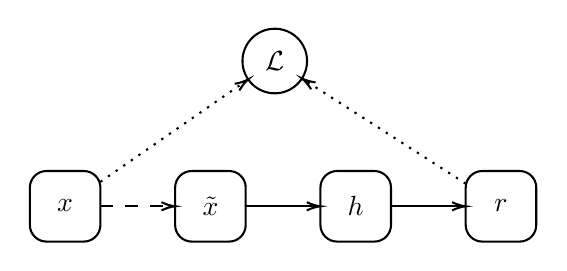
\begin{tikzpicture}[x=0.75pt,y=0.75pt,yscale=-1,xscale=1]
%uncomment if require: \path (0,172); %set diagram left start at 0, and has height of 172


% Text Node
\draw    (136, 40) circle [x radius= 15.56, y radius= 15.56]   ;
\draw (136,40) node   [align=left] {\begin{minipage}[lt]{13.735995849609345pt}\setlength\topsep{0pt}
\begin{center}
$\displaystyle \mathcal{L}$
\end{center}

\end{minipage}};
% Text Node
\draw    (18,101) .. controls (18,96.58) and (21.58,93) .. (26,93) -- (44,93) .. controls (48.42,93) and (52,96.58) .. (52,101) -- (52,119) .. controls (52,123.42) and (48.42,127) .. (44,127) -- (26,127) .. controls (21.58,127) and (18,123.42) .. (18,119) -- cycle  ;
\draw (35,110) node   [align=left] {\begin{minipage}[lt]{20.400000000000002pt}\setlength\topsep{0pt}
\begin{center}
$\displaystyle \boldsymbol{x}$
\end{center}

\end{minipage}};
% Text Node
\draw    (88,101) .. controls (88,96.58) and (91.58,93) .. (96,93) -- (114,93) .. controls (118.42,93) and (122,96.58) .. (122,101) -- (122,119) .. controls (122,123.42) and (118.42,127) .. (114,127) -- (96,127) .. controls (91.58,127) and (88,123.42) .. (88,119) -- cycle  ;
\draw (105,110) node   [align=left] {\begin{minipage}[lt]{20.400000000000002pt}\setlength\topsep{0pt}
\begin{center}
$ $$\displaystyle \boldsymbol{\tilde{x}}$
\end{center}

\end{minipage}};
% Text Node
\draw    (158,101) .. controls (158,96.58) and (161.58,93) .. (166,93) -- (184,93) .. controls (188.42,93) and (192,96.58) .. (192,101) -- (192,119) .. controls (192,123.42) and (188.42,127) .. (184,127) -- (166,127) .. controls (161.58,127) and (158,123.42) .. (158,119) -- cycle  ;
\draw (175,110) node   [align=left] {\begin{minipage}[lt]{20.400000000000002pt}\setlength\topsep{0pt}
\begin{center}
$\displaystyle \boldsymbol{h}$
\end{center}

\end{minipage}};
% Text Node
\draw    (228,101) .. controls (228,96.58) and (231.58,93) .. (236,93) -- (254,93) .. controls (258.42,93) and (262,96.58) .. (262,101) -- (262,119) .. controls (262,123.42) and (258.42,127) .. (254,127) -- (236,127) .. controls (231.58,127) and (228,123.42) .. (228,119) -- cycle  ;
\draw (245,110) node   [align=left] {\begin{minipage}[lt]{20.400000000000002pt}\setlength\topsep{0pt}
\begin{center}
$\displaystyle \boldsymbol{r}$
\end{center}

\end{minipage}};
% Connection
\draw  [dash pattern={on 4.5pt off 4.5pt}]  (52,110) -- (86,110) ;
\draw [shift={(88,110)}, rotate = 180] [color={rgb, 255:red, 0; green, 0; blue, 0 }  ][line width=0.75]    (6.56,-1.97) .. controls (4.17,-0.84) and (1.99,-0.18) .. (0,0) .. controls (1.99,0.18) and (4.17,0.84) .. (6.56,1.97)   ;
% Connection
\draw    (122,110) -- (156,110) ;
\draw [shift={(158,110)}, rotate = 180] [color={rgb, 255:red, 0; green, 0; blue, 0 }  ][line width=0.75]    (6.56,-1.97) .. controls (4.17,-0.84) and (1.99,-0.18) .. (0,0) .. controls (1.99,0.18) and (4.17,0.84) .. (6.56,1.97)   ;
% Connection
\draw    (192,110) -- (226,110) ;
\draw [shift={(228,110)}, rotate = 180] [color={rgb, 255:red, 0; green, 0; blue, 0 }  ][line width=0.75]    (6.56,-1.97) .. controls (4.17,-0.84) and (1.99,-0.18) .. (0,0) .. controls (1.99,0.18) and (4.17,0.84) .. (6.56,1.97)   ;
% Connection
\draw  [dash pattern={on 0.84pt off 2.51pt}]  (52,98.22) -- (121.57,50) ;
\draw [shift={(123.21,48.86)}, rotate = 505.28] [color={rgb, 255:red, 0; green, 0; blue, 0 }  ][line width=0.75]    (6.56,-1.97) .. controls (4.17,-0.84) and (1.99,-0.18) .. (0,0) .. controls (1.99,0.18) and (4.17,0.84) .. (6.56,1.97)   ;
% Connection
\draw  [dash pattern={on 0.84pt off 2.51pt}]  (228,99.08) -- (150.77,49.49) ;
\draw [shift={(149.09,48.41)}, rotate = 392.71000000000004] [color={rgb, 255:red, 0; green, 0; blue, 0 }  ][line width=0.75]    (6.56,-1.97) .. controls (4.17,-0.84) and (1.99,-0.18) .. (0,0) .. controls (1.99,0.18) and (4.17,0.84) .. (6.56,1.97)   ;

\end{tikzpicture}